

In the proposed architecture, the Gateway is the central module of the system, connecting the SmartBoxes to the \acs{HIS}. It's also responsible for the management of devices and their associations (SmartBox - Biosticker), managing, maintaining and storing the data that is generated by these, as well as handling any communication from the \acs{HIS}. The Gateway maintains a list of all the SmartBoxes that are managed by the system, as well as every Biosticker and every sensor in the biosticker (which are used to indicate which ``sensor'' measured the respective biosignal to the \acs{HIS}). 


\section{Services Overview}
\dots 
\section{Data Store}
\dots 


\subsection{Database Schema}
\dots 

\begin{figure}[H]
    \centering
    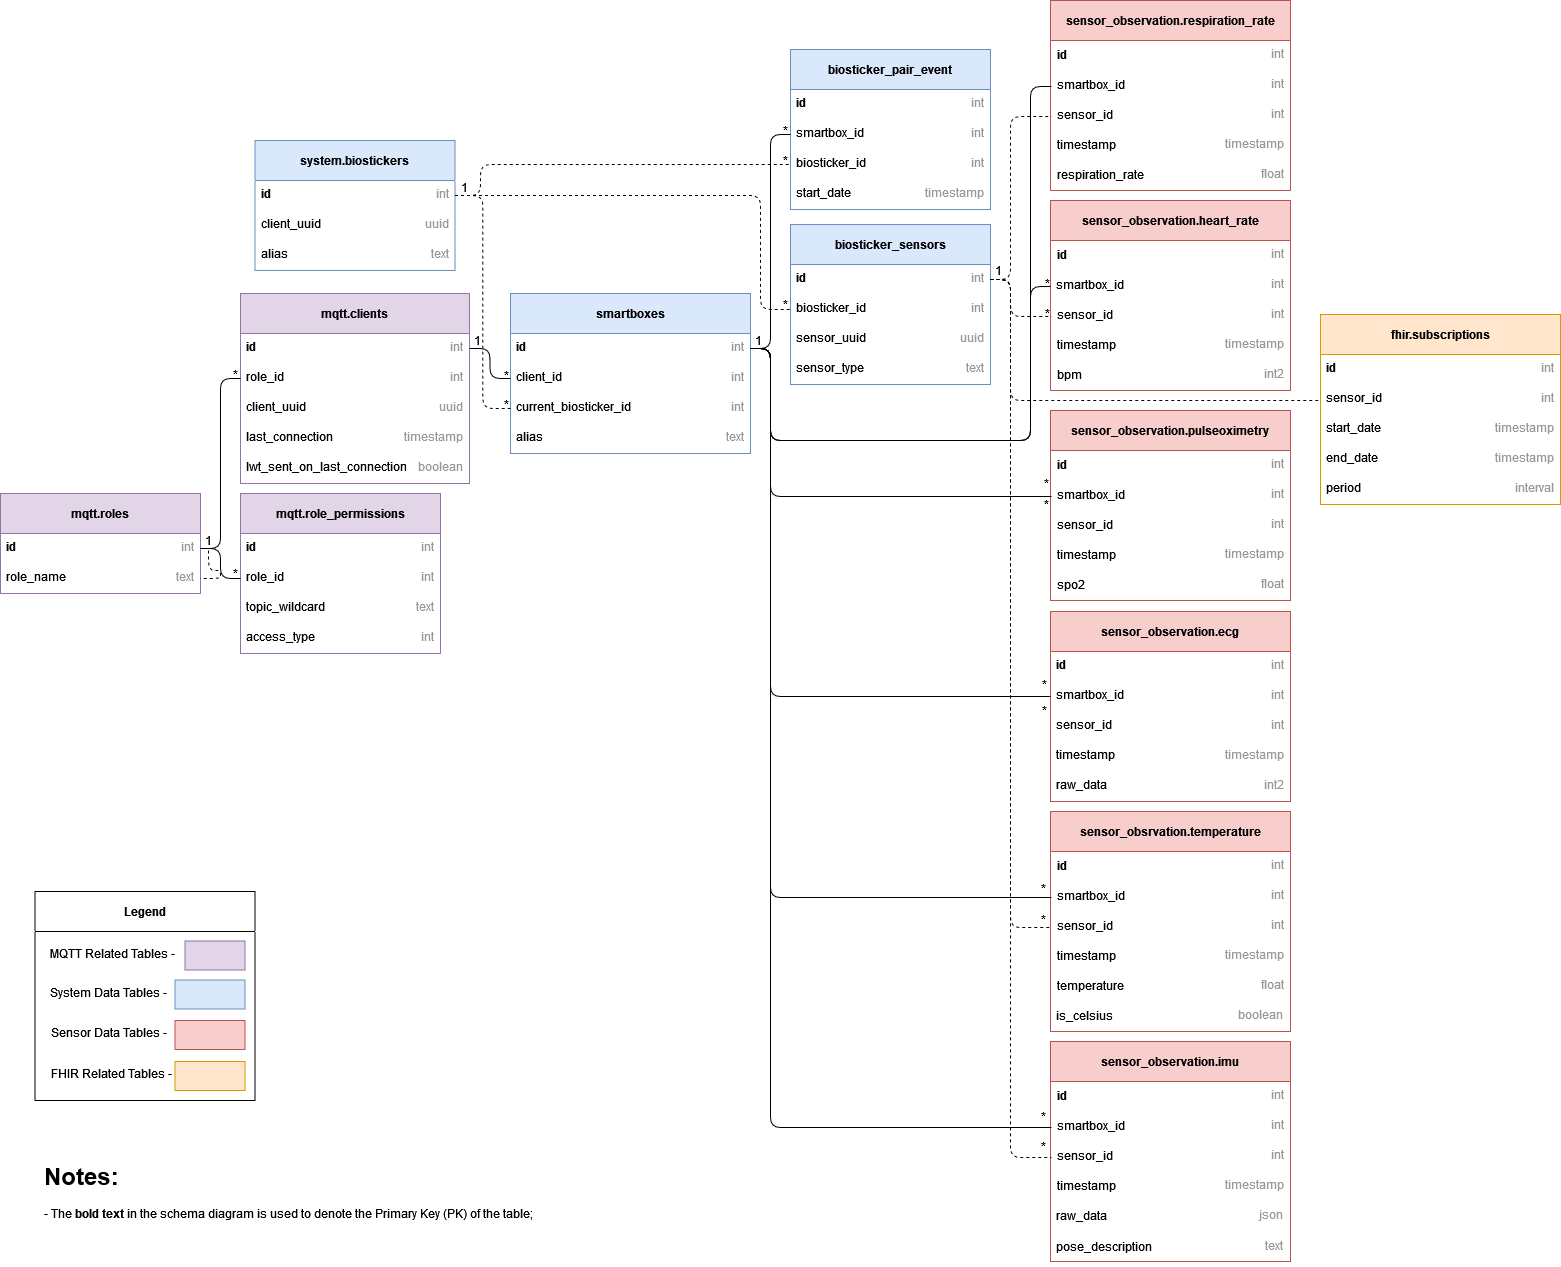
\includegraphics[width=\linewidth]{images/wow-dbschema-full.png}
    \caption[test]{test}
    \label{fig:wow-dbschema-full}
\end{figure}

\subsubsection{MQTT Client Information}
\dots 

\begin{figure}[H]
    \centering
    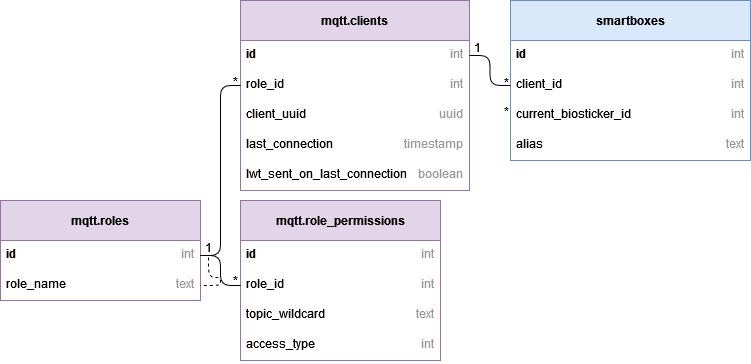
\includegraphics[width=\linewidth]{images/wow-dbschema-mqtt.png}
    \caption[test]{test}
    \label{fig:wow-dbschema-mqtt}
\end{figure}

\subsubsection{Sensor Data}
\dots 

\begin{figure}[H]
    \centering
    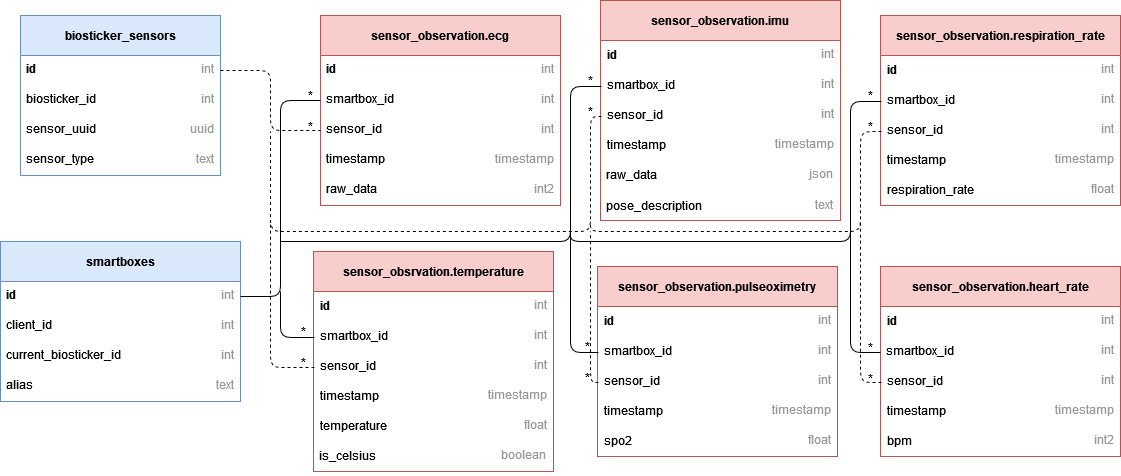
\includegraphics[width=\linewidth]{images/wow-dbschema-sensors.png}
    \caption[test]{test}
    \label{fig:wow-dbschema-sensors}
\end{figure}

\subsubsection{FHIR Related Information}
\dots 

\begin{figure}[H]
    \centering
    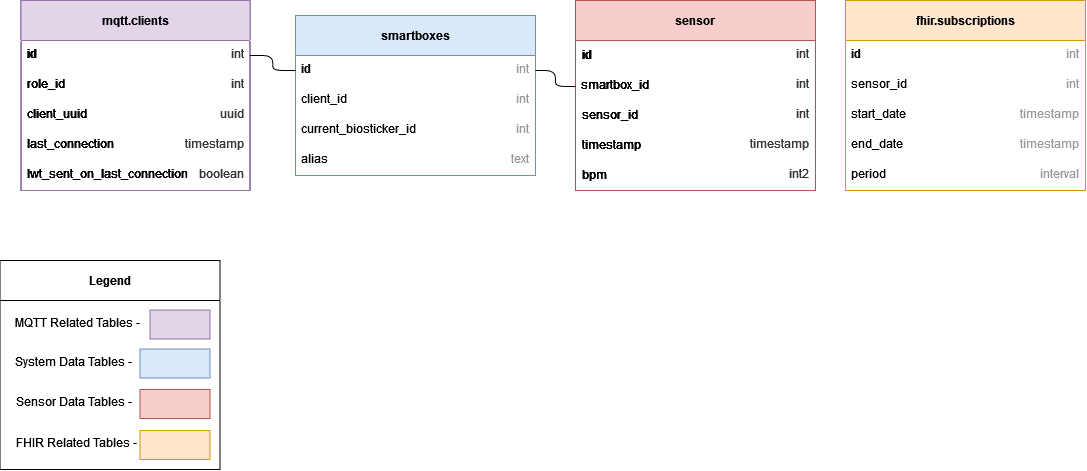
\includegraphics[width=\linewidth]{images/wow-dbschema-fhir.png}
    \caption[test]{test}
    \label{fig:wow-dbschema-fhir}
\end{figure}

\section{Connection to the SmartBoxes}

\section{Integration with GlobalCare}

\section{Summary}
In this chapter, we \dots